\documentclass{beamer}

% import packages
\usepackage[T1]{fontenc}
\usepackage{lmodern}
\usepackage[a0paper]{beamerposter}
\usepackage{graphicx}
\usepackage{booktabs}
\usepackage{tikz}
\usepackage{pgfplots}
\usepackage{anyfontsize}
\usepackage{siunitx}
\usepackage{multicol}

% configure pgfplots
\pgfplotsset{compat=1.14}

% specify theme and color theme
\usetheme{gemini}
\usecolortheme{earth}

% define poster lengths for columns
% If you have N columns, choose \sepwidth and \colwidth such that
% (N+1)*\sepwidth + N*\colwidth = \paperwidth
\newlength{\sepwidth}
\newlength{\colwidth}
\setlength{\sepwidth}{0.025\paperwidth}
\setlength{\colwidth}{0.3\paperwidth}
% define the separator column command
\newcommand{\separatorcolumn}{\begin{column}{\sepwidth}\end{column}}

% configure the author block
\title{Microtubule force generation in axon growth cones}
\author{Calvin Sprouse}
\institute[CWU]{Department of Physics, Central Washington University}

% configure the footer
\footercontent{
    PHYS 322 Computational Biophysics \hfill
    2024 March 12 \hfill
    \href{mailto:calvin.sprouse@cwu.edu}{calvin.sprouse@cwu.edu}
}

% setup logo
\logoright{
\includegraphics[height=7cm]{figures/logos/cwu_logo.png}}


%-----------------------------------------------------------------------------%
% begin poster
\begin{document}

% begin the content framework
\begin{frame}[t]
\begin{columns}[t]
\separatorcolumn%


%-----------------------------------------------------------------------------%
% first column of content
\begin{column}{\colwidth}

%------------------------------------------------
% introduction/abstract block
\begin{block}{Introduction}

The neuron is a class of living cell adapted to function as a network node. Neurons have two types of protrusion from their cell body which begin as neurites. Most neurites become dendrites, which are smaller branches that support bidirectional transport of both signal and cargo. They also serve as targets for incoming network connections from other neurons. One neurite on each neuron becomes the axon. This longer branch is adapted to support outbound signaling from the cell body. While the dendrites remain relatively close to cell body the axon grows following chemical cues. The rate of axon growth varies by the function of the neuron and can extend from micrometers to meters.

Besides its length, the axon expresses unique internal traits from the dendrite. Most notably is the emergent ordering of microtubule (MT) filaments in the axon~\cite{nedelec1997n13}. MTs are dynamic assemblies of tubulin that serve as molecular highways. The plus-end of an MT is where most polymerization activity occurs. The polarity of an MT is its relative orientation in the context of the cell body. Molecular motors are sensitive to polarity as each motor has a directional preference. Dynein, for example, is a minus-directed motor and walks away from the plus-end. Kinesin, on the other hand, is a plus-directed motor. The polarity pattern describes the spatial distribution of MT polarity and indicates the function of the region.

\begin{figure}
    \centering
    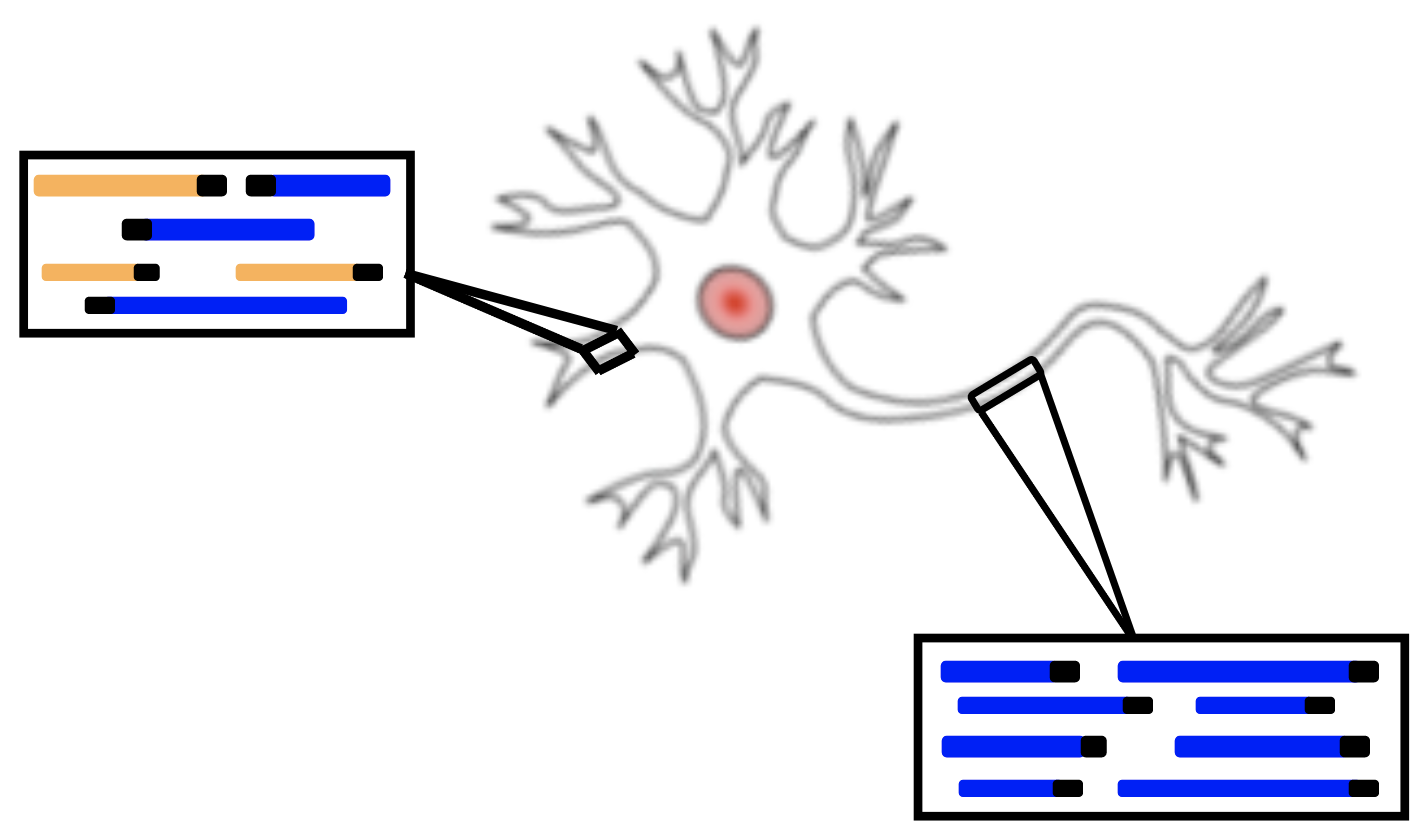
\includegraphics[width=0.5\textwidth]{figures/background/neuron_with_mts.png}
    \caption{\label{fig:neuron_background}
        A neuron with dendrites and an axon extending from the cell body. MTs are shown in two regions: left is a dendrite, and right is an axon. The plus-end of the MTs is indicated by a black rectangle. The orientation of the MTs with respect to the cell body is indicated by the color: blue MTs are plus-end-out, orange MTs are minus-end-out.}
\end{figure}

The axon shown in Figure~\ref{fig:neuron_background} expresses the typical plus-end-out polarity pattern whereas the dendrite exhibits a typical mixed polarity pattern.

\end{block}

\begin{block}{Background}

\begin{figure}
    \centering
    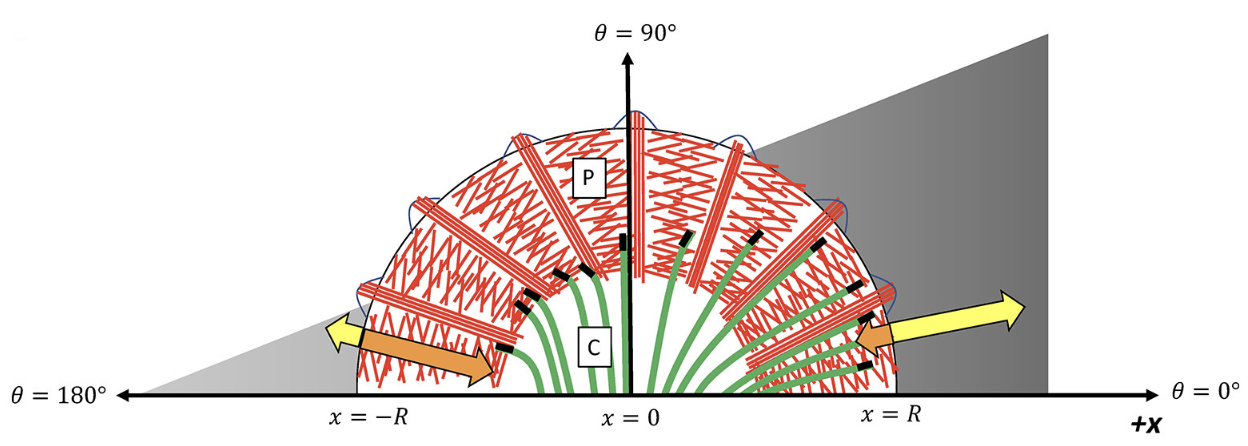
\includegraphics[width=0.65\textwidth]{figures/introduction/gc_crag_1a.png}
    \caption{\label{fig:gc_craig}
        Illustrative schematic of a growth cone from Ref.~\cite{craig2018fcn} Figure 1A. Shown in green with black tips are the MTs as in Figure~\ref{fig:neuron_background}. Shown in black is a chemical gradient indicating the direction the GC should steer. Yellow and orange arrows indicate the relative velocity of forward polymerization and depolymerization respectively of the actomyosin network. The presence of MTs increases adhesion of the actomyosin network and promotes forward polymerization.
    }
\end{figure}

Axon growth is lead by a region called the growth cone (GC) shown in Figure~\ref{fig:gc_craig}. The GC is distinguished from the rest of the axon by a decrease in MT density, sensing equipment for reading chemical guidance cues, and a force generating network of actin filaments and myosin motors.

\begin{figure}
    \centering
    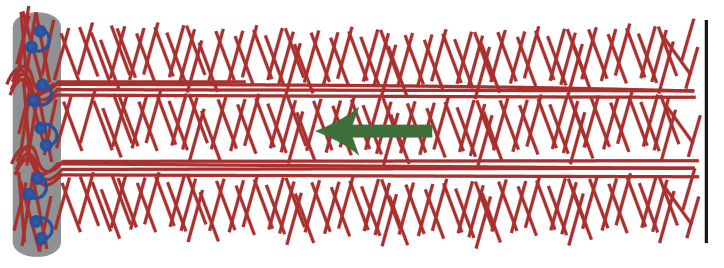
\includegraphics[width=0.4\textwidth]{figures/introduction/actin_treadmill.png}
    \caption{\label{fig:actin_craig}
        Actin treadmill schematic from Ref.~\cite{craig2012bj} Figure 1B. This view is effectively a thin angular slice of Figure~\ref{fig:gc_craig}. The rightmost edge is the leading edge of the GC where polymerization activity occurs. The leftmost edge then houses the depolymerization machinery.
    }
\end{figure}

The actomyosin network is a treadmill of actin filaments and myosin motors thought to be the primary diver in elongation~\cite{craig2012bj}. The treadmill behavior emerges from the combination of leading edge polymerization and trailing edge depolymerization of the actin shown in Figure~\ref{fig:actin_craig}. Also impacting the actomyosin network are tension forces from the stretching of the GC membrane~\cite{craig2012bj}. Myosin acts simultaneously as a crosslinker for the network and the transporter of trailing edge depolymerize actin filament to the leading edge for polymerization. By modulating actin adhesion to the substrate the GC can execute carefully controlled growth and steering. The role of MTs is currently understood as signal pathways between the chemical sensing equipment and the actomyosin network~\cite{craig2012bj, kalil2005con, sanchez-huertas2021fmn}.

\begin{figure}
    \centering
    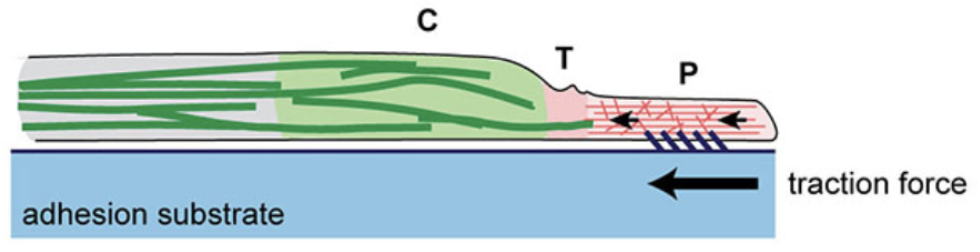
\includegraphics[width=0.5\textwidth]{figures/introduction/traction_generation.png}
    \caption{\label{fig:traction}
        A side-view schematic of the GC from Ref.~\cite{athamneh2015fcn} Figure 1. Shown in green are the MTs as in Figure~\ref{fig:neuron_background}. This is representative of our proposed one-dimensional model. Black arrows indicate the direction of actin flow and generated forces from the GC frame.
    }
\end{figure}

We investigate the role of the MTs in the GC regions as conveyors of force from the axon. In the axon, Dynein motors act between MTs inducing \(\qty{}{\pico\newton}\) scale forces primarily in the direction of the MTs plus-end~\cite{nedelec1997n13, raffa2023scdb}. The forces acting on the GC are observed to be small, on the order of \(\qty{}{\pico\newton}\)~\cite{devincentiis2020jn, raffa2023scdb}. Furthermore, it seems the MTs protruding into the GC act to stabilize against contractile forces generated in the actomyosin network and the GC membrane~\cite{raffa2023scdb}. We extend the work done in Ref.~\cite{craig2012bj} to include distill-end MT force generation by a Dynein sorting mechanism and investigate the consequence of interaction in the GC.

\end{block}

\end{column}
\separatorcolumn%


%-----------------------------------------------------------------------------%
% second column of content
\begin{column}{\colwidth}

%------------------------------------------------
% content block
\begin{block}{Model}

We begin with Ref.~\cite{craig2012bj} which describes a one-dimensional computational adhesion clutch model in the context of the actomyosin network. This is a population based steady-state model which aims to explore the relationship of actin retrograde flow, actin density, and traction forces.

% "default" figure from simulation showing exactly this relationship
\begin{figure}
    \centering
    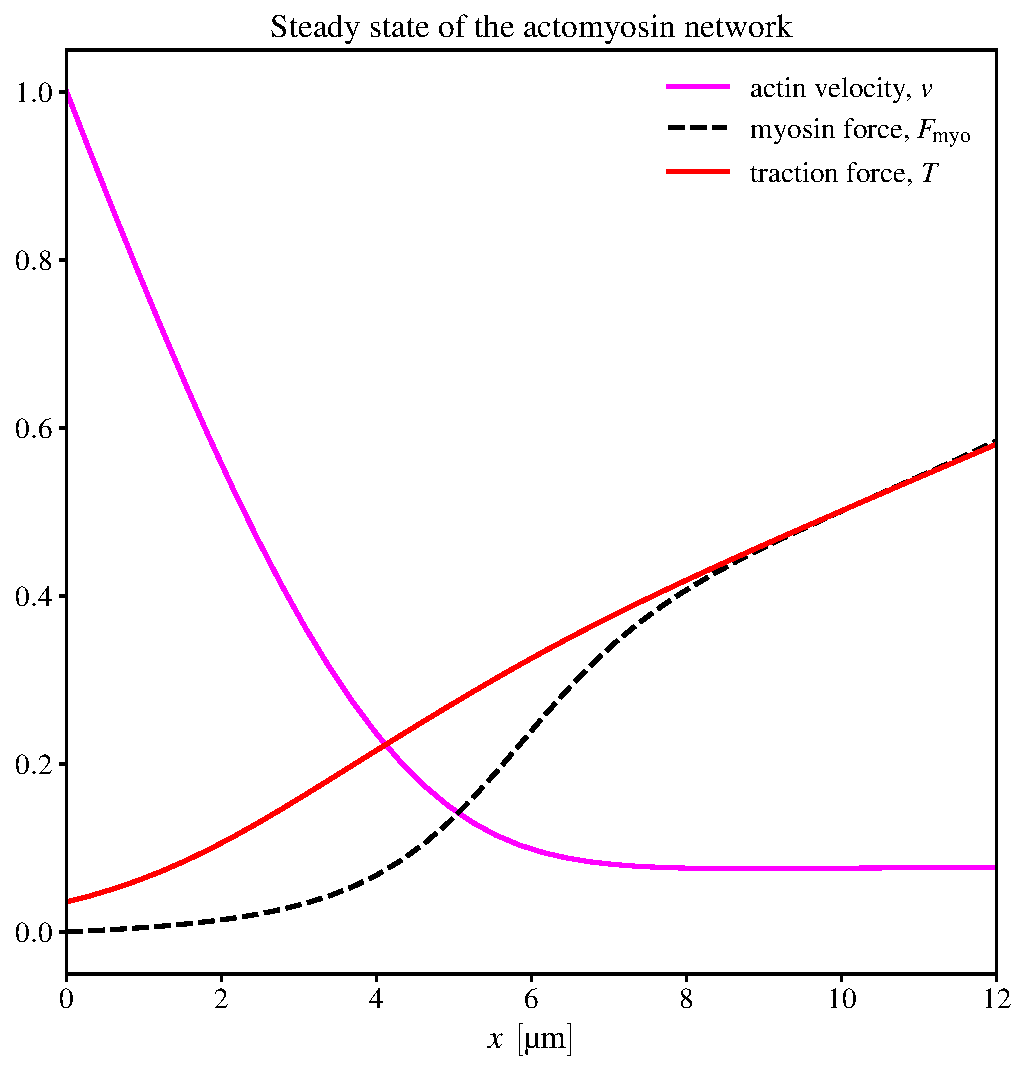
\includegraphics[width=0.35\textwidth]{../.figures/steady_state_og.pdf}
    \caption{\label{fig:sim_steady}
        Representative output of the steady state of the actomyosin network from Ref.~\cite{craig2012bj}. The pink line represents the retrograde actin flow speed from the leading edge, \(x=\qty{0}{\micro\meter}\), to the trailing edge, \(x=\qty{12}{\micro\meter}\). The black dashed line represents the contractile forces from myosin. The red line represents the traction forces arising from actin adhesion to the substrate. Under these conditions the GC is moving in the \(-x\) direction.
    }
\end{figure}

In addition to the features of this model we introduce MTs protruding from the axon via Dynein sliding forces. After the network has reached a steady state, we permit MTs to enter the GC through Dynein sliding forces and MT polymerization. Here we introduce two distinct behaviors for testing:
\begin{enumerate}
\item crosslinker proteins bind primarily to the plus-end of the MT effectively resulting in a single point of contact with the actomyosin network;
\item crosslinker proteins bind uniformly to the MT resulting in multiple contact points across the actomyosin network.
\end{enumerate}

% model figure
\begin{figure}
    \centering
    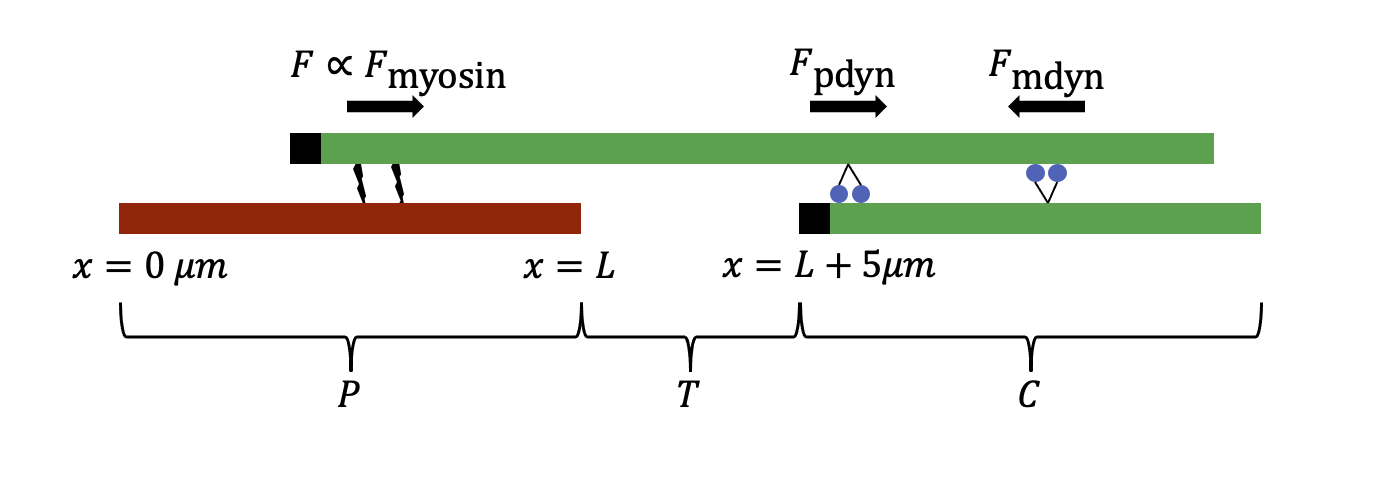
\includegraphics[width=0.9\textwidth]{figures/model/model.png}
    \caption{\label{fig:main_model}
        The one-dimensional model of the GC under study. Labelled below are the P, T, and C regions of the GC. In the P region we model an actomyosin network as in Ref.~\cite{craig2012bj}. Here, crosslinker proteins bind to the protruding MT and exert a force proportional to the velocity of myosin at the binding location. The length of this region can be tuned but it set to \(L=\qty{12}{\micro\meter}\). In the \(\qty{5}{\micro\meter}\) T region no protein binding occurs. In the C region Dynein motors bind between the single MT protruding into the GC and an array of axonal MTs assumed to be stabilized against motion by a network of crosslinkers.
    }
\end{figure}

The simulation begins with the actomyosin network reaching a steady state as described by Ref.~\cite{craig2012bj}. Once in a steady state we move to an agent based model simulating the action of a single MT protruding into the GC. We simulate the interactions of this MT and motor proteins described in Figure~\ref{fig:main_model} over a characteristic time of \(t=\qty{100}{\second}\). This time is obtained by calculating the time it takes for an actin filament to traverse the actomyosin network.

\end{block}

%------------------------------------------------
% content block
\begin{block}{Results}

Results, what did this tell us.

\end{block}

\end{column}
\separatorcolumn%


%-----------------------------------------------------------------------------%
% third column of content
\begin{column}{\colwidth}

%------------------------------------------------
% content block
\begin{block}{Results}

Results, what did this tell us.

\end{block}

%------------------------------------------------
% future work block
\begin{block}{Future Work}

This model is constructed on a population based steady state model with temporal attributes included as an after-thought. A more rigorous approach would likely include an agent based model with mt motions, protein binding events, and actin network activity taking place with defined rates. An agent based simulation constructed in this way could explore more precise relationships between actin treadmilling, adhesion, and mt force generation by sliding and polymerization. Constructed properly, this agent based simulation could explore the two-dimensional landscape of the growth cone and investigate the role of mt force generation in growth cone guidance or lack thereof. Furthermore, such a model would have the advantage of being double validated by the original population model in the growth cone and agent based simulations in the axon.

\end{block}

%------------------------------------------------
% reference block
\begin{block}{References}
\begin{multicols}{2}
\fontsize{16pt}{12pt}\selectfont
\nocite{craig2015pb, craig2012bj, devincentiis2020jn, kalil2005con, nedelec1997n13, raffa2023scdb, sanchez-huertas2021fmn}
\bibliographystyle{plain}
\bibliography{../proposal/axon_growth2.bib}
\end{multicols}
\end{block}

\end{column}
\separatorcolumn%

\end{columns}
\end{frame}
\end{document}
